\section{Cellular and homological transition identities}\label{sec:homology}
Let $D\subseteq D'$ be occurrence sets, $K=K(D)$, $K'=K(D')$, $K^\circ=K\cap K'=K\setminus\mathrm{Dead}$ and $\mathrm{New}=K'\setminus K$ as in \cref{thm:A5T32}. Homology is taken over a field $\mathbb k$ ($\F_2$ for all computations; the proofs hold over any field). Write $\beta_i,\beta_i'$ for the Betti numbers of $K,K'$, $\mathrm{Dead}_i,\mathrm{New}_i$ for the sets of $i$-cells, and, for the inclusions $\iota:K^\circ\to K$, $\iota':K^\circ\to K'$,
\[
\begin{aligned}r_i&=\rank(\iota_*:H_i(K^\circ)\to H_i(K)),& r_i'&=\rank(\iota'_*:H_i(K^\circ)\to H_i(K')),\\ h_i&=\dim H_i(K,K^\circ),& h_i'&=\dim H_i(K',K^\circ),\end{aligned}
\]
with the convention that all quantities of negative degree vanish. The \emph{zig-zag} $K\hookleftarrow K^\circ\hookrightarrow K'$ compares the two complexes through what survives. It is a diagram of the shape studied in zigzag persistence~\cite{CarlssonDeSilva2010} (see also~\cite{CarlssonZomorodian2009}); for this two-step case we need only the long exact sequence of a pair, and the identities below are proved directly from it.

\subsection{The zig-zag identity}
\begin{theorem}[zig-zag identity]\label{thm:zigzag}
For every $i\ge0$,
\[
\beta_i(K)=r_i+h_i-\beta_{i-1}(K^\circ)+r_{i-1},\qquad \beta_i(K')=r_i'+h_i'-\beta_{i-1}(K^\circ)+r_{i-1}',
\]
and therefore
\[
\Delta\beta_i:=\beta_i'-\beta_i=(h_i'-h_i)+(r_i'-r_i)+(r_{i-1}'-r_{i-1}).
\]
Moreover $\Delta\chi=\chi(K')-\chi(K)=\sum_i(-1)^i(|\mathrm{New}_i|-|\mathrm{Dead}_i|)$ is local: it depends only on the dead and new cells.
\end{theorem}
\prov{CW-0444}{A5-T4.1}{PROVED}{FULL}
\begin{proof}
The long exact sequence of the pair $(K,K^\circ)$ reads $\cdots\to H_i(K^\circ)\xrightarrow{\iota_*}H_i(K)\to H_i(K,K^\circ)\xrightarrow{\partial}H_{i-1}(K^\circ)\xrightarrow{\iota_*}H_{i-1}(K)\to\cdots$. By exactness, $\dim H_i(K)=\operatorname{rank}\iota_*+\operatorname{rank}(H_i(K)\to H_i(K,K^\circ))$, and the second rank equals $\dim\ker\partial=h_i-\operatorname{rank}\partial$. Again by exactness $\operatorname{rank}\partial=\dim\ker(\iota_*:H_{i-1}(K^\circ)\to H_{i-1}(K))=\beta_{i-1}(K^\circ)-r_{i-1}$. This gives the first formula; the second is the same argument for the pair $(K',K^\circ)$. Subtracting, the terms $\beta_{i-1}(K^\circ)$ cancel. For $\chi$: $K=K^\circ\sqcup\mathrm{Dead}$ and $K'=K^\circ\sqcup\mathrm{New}$ as sets of cells. \qedhere
\end{proof}
\begin{remark}[what is local]
The numbers $h_i,h_i'$ are homology of the relative chain complexes of the dead and new cells modulo $K^\circ$; $r_i,r_i'$ depend on how the surviving complex sits in $K$ and in $K'$. Everything is determined by $(D,D')$ through the rule of \cref{thm:A5T31}.
\end{remark}
\begin{example}[the piercing event of \cref{ex:interval}]\label{ex:zigzag}
$K=K(\{8,22,176\})$ is a triangle with $\beta=(1,1)$; all three edges die, so $K^\circ$ is three points, $\beta(K^\circ)=(3,0)$. Then $r=(1,0)$ (three points map onto one component) and $h=(0,3)$ (three relative $1$-cells). $K'$ has $f=(9,11,3)$ and $\beta'=(1,0)$, with $r'=(1,0)$ and $h'=(0,2)$. The identity gives $\Delta\beta_1=(2-3)+(0-0)+(1-1)=-1$ and $\Delta\beta_0=0$, as observed (\cref{fig:zigzag}). The Euler characteristic is local: $|\mathrm{Dead}|=(0,3,0)$, $|\mathrm{New}|=(6,11,3)$, so $\Delta\chi=(6-0)-(11-3)+(3-0)=1=\chi(K')-\chi(K)=1-0$. Chain-level boundary matrices and the check $\partial^2=0$ are in Appendix~\ref{app:homology}.
\end{example}
\begin{figure}[tbp]\centering
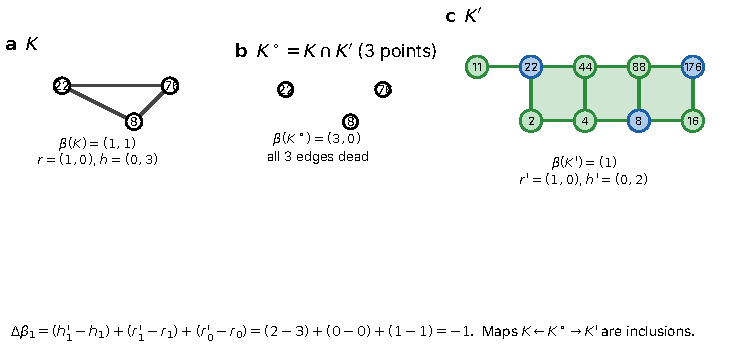
\includegraphics[width=\textwidth]{fig20_zigzag}
\caption{\textbf{The zig-zag $K\hookleftarrow K^\circ\hookrightarrow K'$ for the event of \cref{ex:interval} (exact; \cref{thm:zigzag}).} Left: $K(\{8,22,176\})$, a triangle, $\beta=(1,1)$. Centre: $K^\circ=K\cap K'$, the three surviving vertices (all three edges are dead), $\beta=(3,0)$. Right: $K(D')$, $f=(9,11,3)$, $\beta=(1,0)$. The numbers $r,h,r',h'$ of the identity are listed under the panels. The drawing is schematic (abstract layout of the complexes); the embedded version is \cref{fig:beforeafter}.}\label{fig:zigzag}
\end{figure}

\subsection{Which cells cause a change}
\begin{theorem}[cause criteria]\label{thm:cause}
For every $i\ge0$:
\begin{enumerate}[label=(\roman*),itemsep=1pt]
\item if $\Delta\beta_i<0$ then $\mathrm{Dead}_i\ne\emptyset$ or $\mathrm{New}_{i+1}\ne\emptyset$ (a cell of dimension $i$ died or a cell of dimension $i+1$ appeared);
\item if $\Delta\beta_i>0$ then $\mathrm{New}_i\ne\emptyset$ or $\mathrm{Dead}_{i+1}\ne\emptyset$.
\end{enumerate}
In particular, if no cell dies, $\Delta\beta_i<0$ forces a new $(i+1)$-cell.
\end{theorem}
\prov{CW-0445}{A5-T4.2}{PROVED}{FULL}
\begin{proof}
(i) Suppose $\mathrm{Dead}_i=\emptyset=\mathrm{New}_{i+1}$. Then $C_i(K)=C_i(K^\circ)\subseteq C_i(K')$, so $Z_i(K)\subseteq Z_i(K')$ (boundaries of cells of $K^\circ$ are computed in $K^\circ$), and $C_{i+1}(K')=C_{i+1}(K^\circ)\subseteq C_{i+1}(K)$, so $B_i(K')\subseteq B_i(K)$. Hence $\beta_i'=\dim Z_i(K')-\dim B_i(K')\ge\dim Z_i(K)-\dim B_i(K)=\beta_i$, i.e.\ $\Delta\beta_i\ge0$. (ii) Symmetrically, if $\mathrm{New}_i=\emptyset=\mathrm{Dead}_{i+1}$ then $C_i(K')\subseteq C_i(K)$, $C_{i+1}(K)\subseteq C_{i+1}(K')$, so $Z_i(K')\subseteq Z_i(K)$ and $B_i(K)\subseteq B_i(K')$ and $\beta_i'\le\beta_i$. \qedhere
\end{proof}
\begin{remark}[correction of the inherited proof]
The inherited argument for the first part used the equality $B_i(K')=B_i(K)$ when no $(i+1)$-cell is added; that is false when cells die at level $i+1$. The inclusions $Z_i(K)\subseteq Z_i(K')$ and $B_i(K')\subseteq B_i(K)$ used above are what the argument needs, and the statement is unchanged.
\end{remark}
\begin{theorem}[nested events]\label{thm:nested}
If $\mathrm{Dead}=\emptyset$ (so $K\subseteq K'$), then with $k_i=\dim\ker(H_i(K)\to H_i(K'))$ one has
\[
\Delta\beta_i=h_i(K',K)-k_i-k_{i-1}.
\]
\end{theorem}
\prov{CW-0446}{A5-T4.3}{PROVED}{FULL}
\begin{proof}
Here $K^\circ=K$, hence $h=0$, $r_i=\beta_i$ and $r_i'=\beta_i-k_i$. Substitute in \cref{thm:zigzag}. \qedhere
\end{proof}
\begin{remark}[scope]
The nested case occurs along the towers of \cref{sec:towertop} (where $\mathrm{Dead}=\emptyset$ at every tower step), but not in general along orbits: an occurrence event with $\mathrm{Dead}\ne\emptyset$ is a genuine zig-zag (\cref{ex:zigzag}).
\end{remark}
